\newpage
\section{Feldman-Cousins throw distributions}\label{sec:fc_appendix}

\begin{figure*}[htbp]
  \centering
  \subfloat[24 ktMWyr] {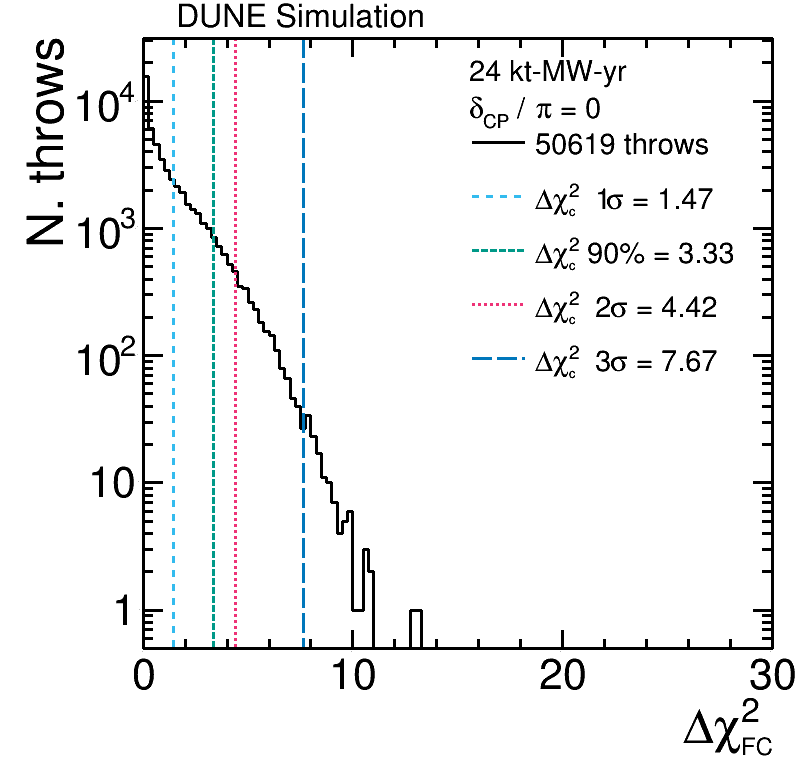
\includegraphics[width=0.33\linewidth]{nh_FC_ndfd_24ktMWyr_dcp0.png}}
  \subfloat[66 ktMWyr] {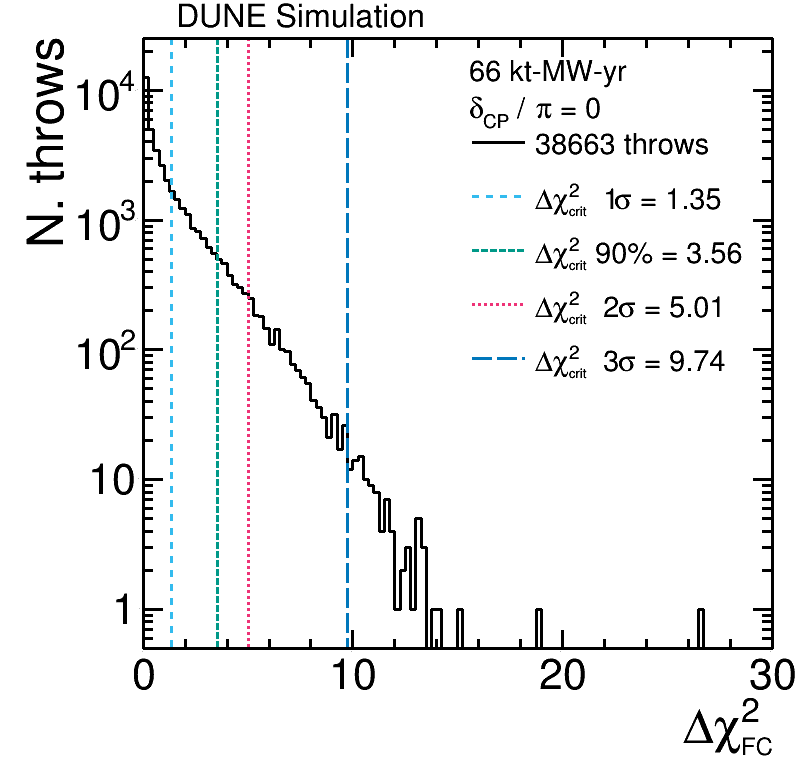
\includegraphics[width=0.33\linewidth]{nh_FC_ndfd_66ktMWyr_dcp0.png}}
  \subfloat[100 ktMWyr]{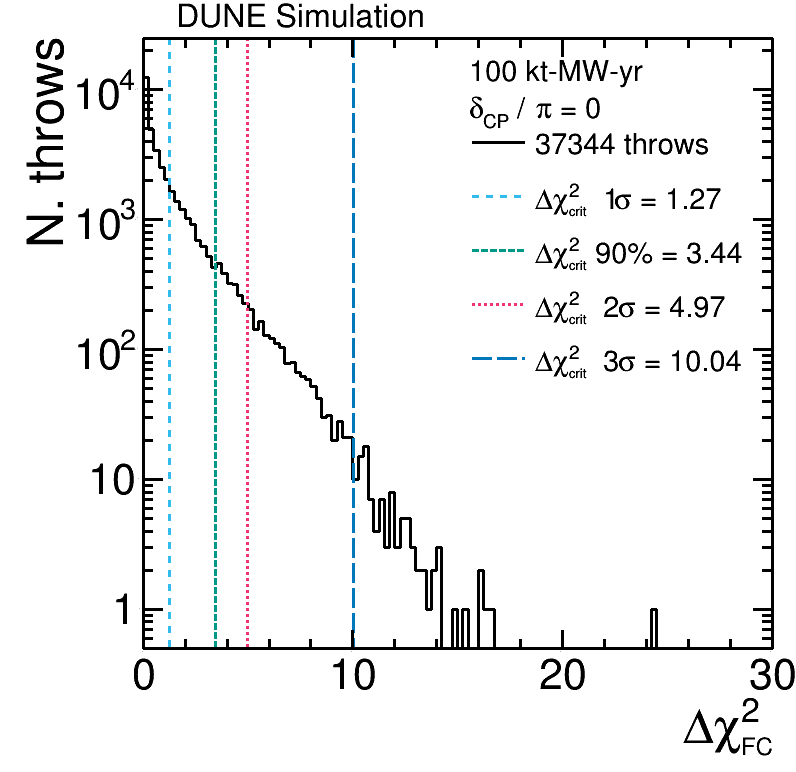
\includegraphics[width=0.33\linewidth]{nh_FC_ndfd_100ktMWyr_dcp0.png}}\\
  \subfloat[150 ktMWyr]{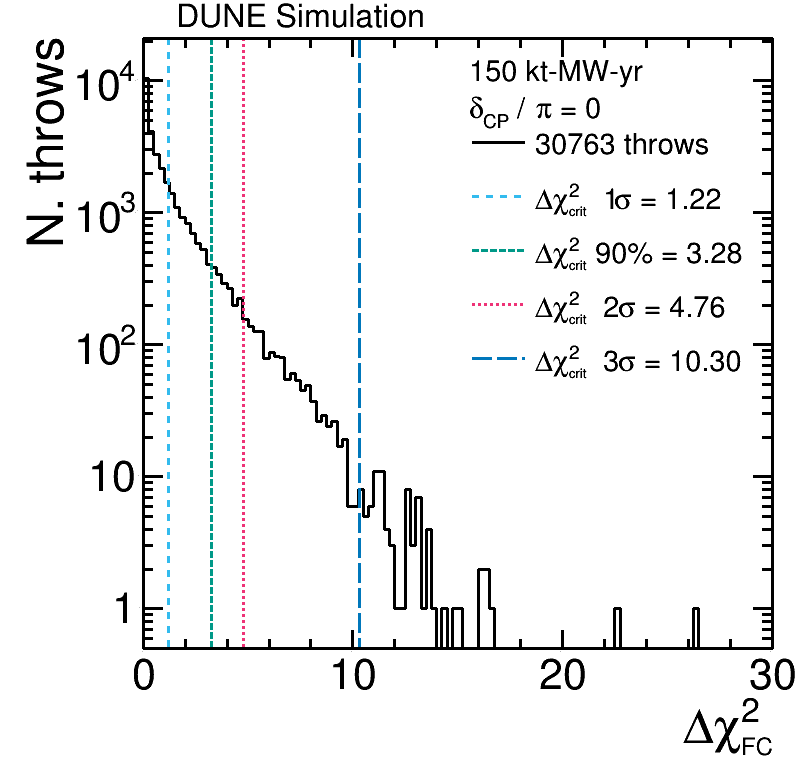
\includegraphics[width=0.33\linewidth]{nh_FC_ndfd_150ktMWyr_dcp0.png}}
  \subfloat[197 ktMWyr]{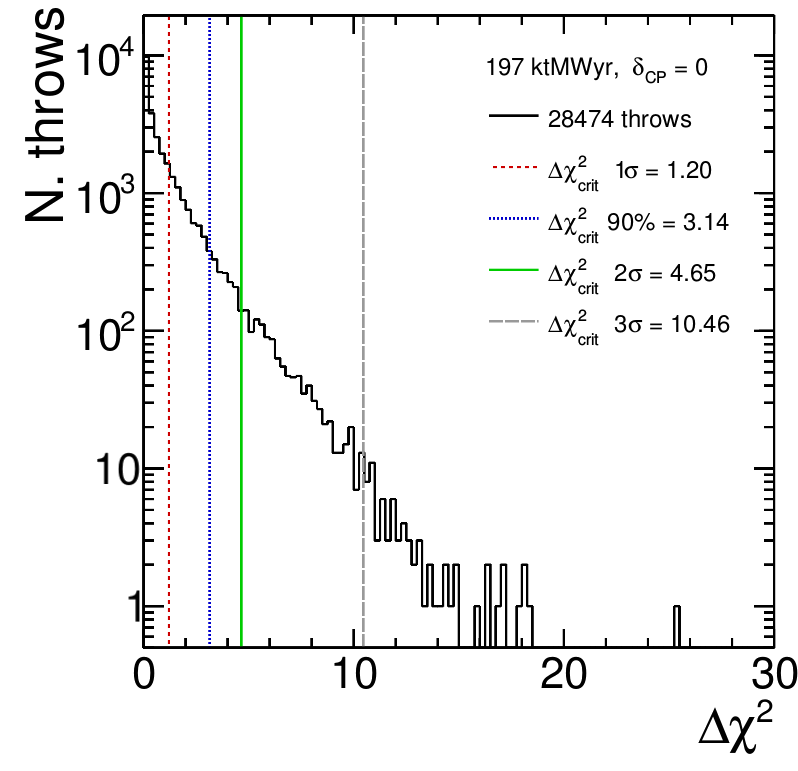
\includegraphics[width=0.33\linewidth]{nh_FC_ndfd_197ktMWyr_dcp0.png}}
  \subfloat[336 ktMWyr]{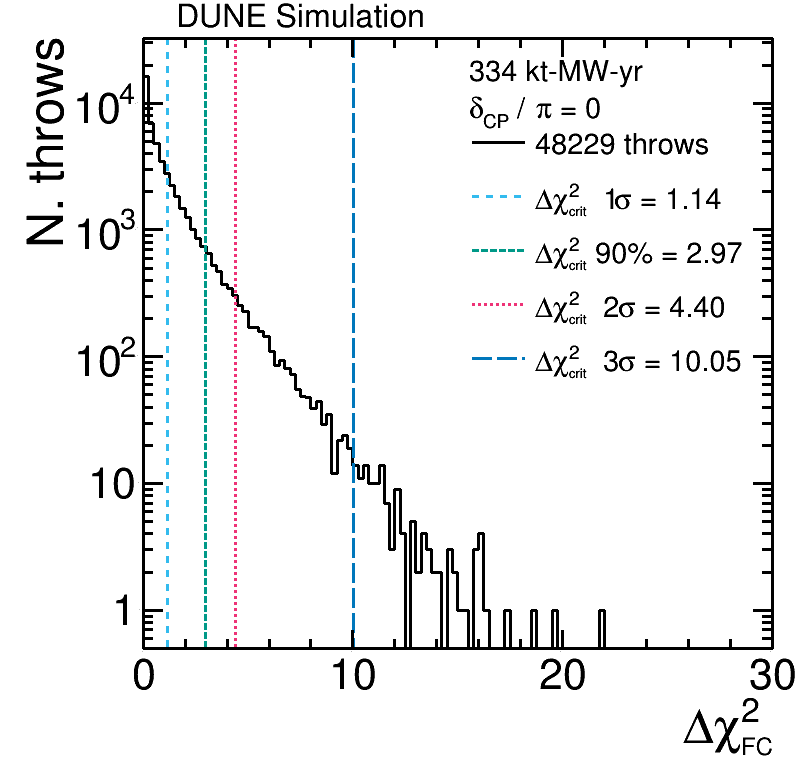
\includegraphics[width=0.33\linewidth]{nh_FC_ndfd_334ktMWyr_dcp0.png}}\\
  \subfloat[500 ktMWyr]{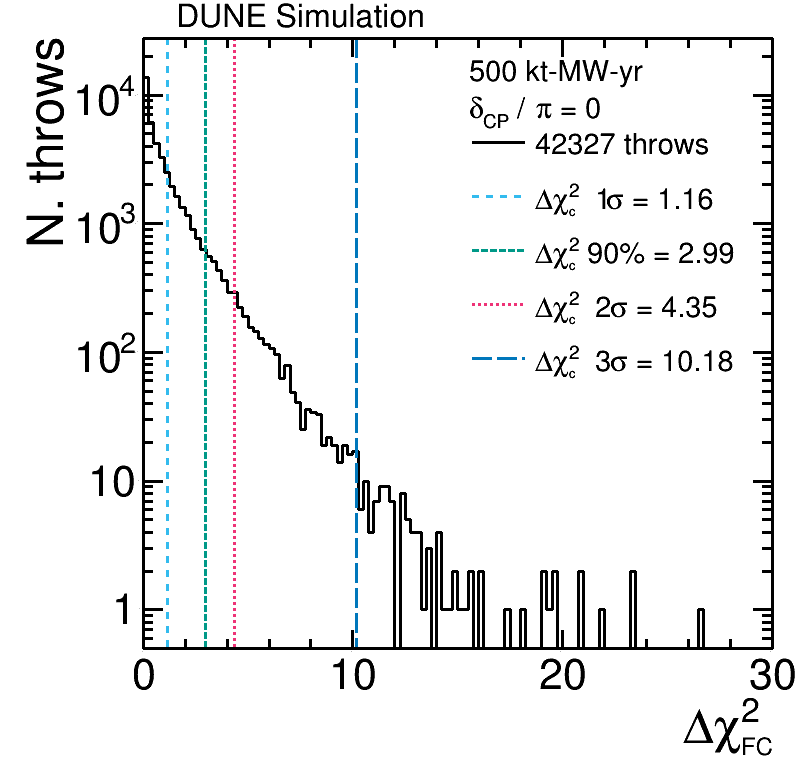
\includegraphics[width=0.33\linewidth]{nh_FC_ndfd_500ktMWyr_dcp0.png}}
  \subfloat[646 ktMWyr]{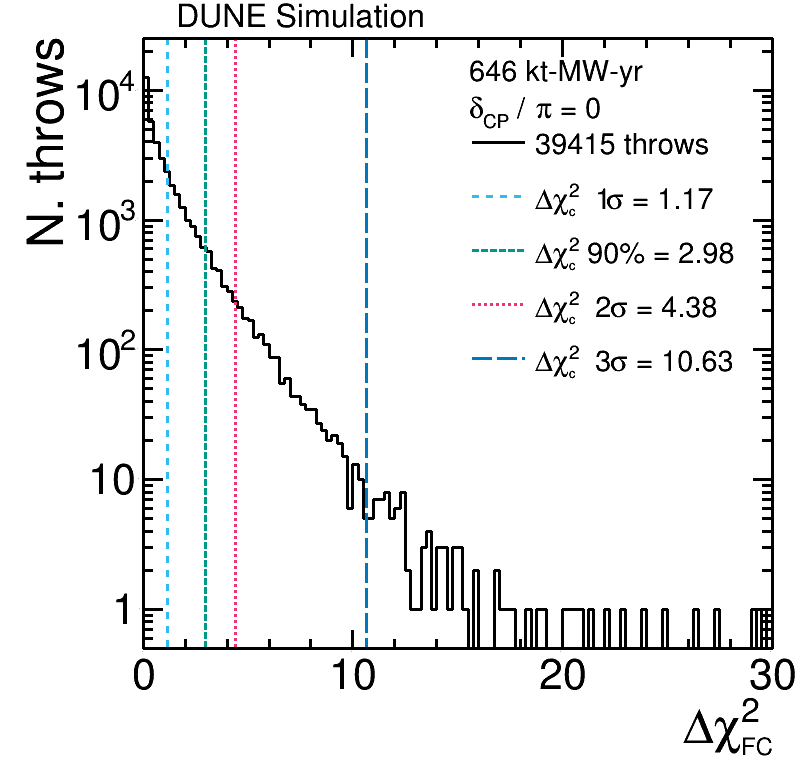
\includegraphics[width=0.33\linewidth]{nh_FC_ndfd_646ktMWyr_dcp0.png}}
  \subfloat[936 ktMWyr]{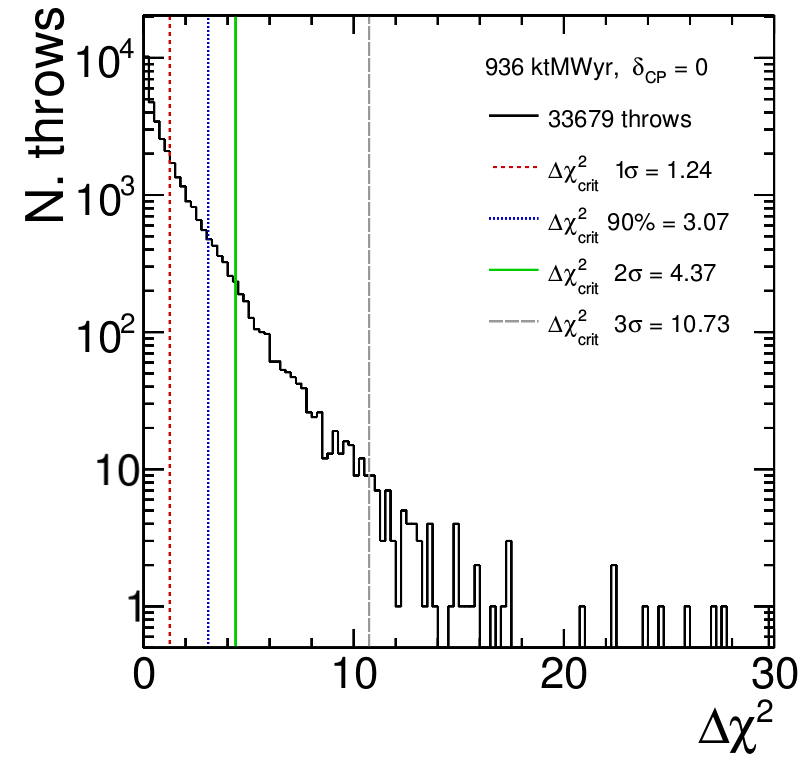
\includegraphics[width=0.33\linewidth]{nh_FC_ndfd_936ktMWyr_dcp0.png}}
  \caption{Distribution of \dchisq values, calculated using Equation~\ref{eq:dchisq_fc}, for a large number of throws with true $\deltacp = 0$, for a variety of exposures. The \dchisqcrit values (vertical lines) obtained using the Feldman-Cousins method show the \dchisq value below which 68.27\% (1$\sigma$), 90\%, 95.45\% (2$\sigma$) and 99.73\% (3$\sigma$) of throws reside, with the calculated values given in the legend. The number of throws used is also given.}
  \label{fig:fc_throws_exp}
\end{figure*}

\begin{figure*}[htbp]
  \centering
  \subfloat[$\deltacp/\pi = -1$]    {\includegraphics[width=0.33\linewidth]{{nh_FC_ndfd_100ktMWyr_dcp-1}.png}}
  \subfloat[$\deltacp/\pi = -0.75$] {\includegraphics[width=0.33\linewidth]{{nh_FC_ndfd_100ktMWyr_dcp-0.75}.png}}
  \subfloat[$\deltacp/\pi = -0.5$]  {\includegraphics[width=0.33\linewidth]{{nh_FC_ndfd_100ktMWyr_dcp-0.5}.png}}\\
  \subfloat[$\deltacp/\pi = -0.25$] {\includegraphics[width=0.33\linewidth]{{nh_FC_ndfd_100ktMWyr_dcp-0.25}.png}}
  \subfloat[$\deltacp/\pi = 0$]     {\includegraphics[width=0.33\linewidth]{{nh_FC_ndfd_100ktMWyr_dcp0}.png}}
  \subfloat[$\deltacp/\pi = 0.25$]  {\includegraphics[width=0.33\linewidth]{{nh_FC_ndfd_100ktMWyr_dcp0.25}.png}}\\
  \subfloat[$\deltacp/\pi = 0.5$]   {\includegraphics[width=0.33\linewidth]{{nh_FC_ndfd_100ktMWyr_dcp0.5}.png}}
  \subfloat[$\deltacp/\pi = 0.75$]  {\includegraphics[width=0.33\linewidth]{{nh_FC_ndfd_100ktMWyr_dcp0.75}.png}}
  \subfloat[$\deltacp/\pi = 1$]     {\includegraphics[width=0.33\linewidth]{{nh_FC_ndfd_100ktMWyr_dcp1}.png}}
  \caption{Distribution of \dchisq values, calculated using Equation~\ref{eq:dchisq_fc}, for a large number of throws for 9 different values of true \deltacp, for a 100 ktMWyr exposure. The \dchisqcrit values (vertical lines) obtained using the Feldman-Cousins method show the \dchisq value below which 68.27\% (1$\sigma$), 90\%, 95.45\% (2$\sigma$) and 99.73\% (3$\sigma$) of throws reside, with the calculated values given in the legend. The number of throws used is also given.}
  \label{fig:fc_throws_100ktMWyr}
\end{figure*}

\begin{figure*}[htbp]
  \centering
  \subfloat[$\deltacp/\pi = -1$]    {\includegraphics[width=0.33\linewidth]{{nh_FC_ndfd_334ktMWyr_dcp-1}.png}}
  \subfloat[$\deltacp/\pi = -0.75$] {\includegraphics[width=0.33\linewidth]{{nh_FC_ndfd_334ktMWyr_dcp-0.75}.png}}
  \subfloat[$\deltacp/\pi = -0.5$]  {\includegraphics[width=0.33\linewidth]{{nh_FC_ndfd_334ktMWyr_dcp-0.5}.png}}\\
  \subfloat[$\deltacp/\pi = -0.25$] {\includegraphics[width=0.33\linewidth]{{nh_FC_ndfd_334ktMWyr_dcp-0.25}.png}}
  \subfloat[$\deltacp/\pi = 0$]     {\includegraphics[width=0.33\linewidth]{{nh_FC_ndfd_334ktMWyr_dcp0}.png}}
  \subfloat[$\deltacp/\pi = 0.25$]  {\includegraphics[width=0.33\linewidth]{{nh_FC_ndfd_334ktMWyr_dcp0.25}.png}}\\
  \subfloat[$\deltacp/\pi = 0.5$]   {\includegraphics[width=0.33\linewidth]{{nh_FC_ndfd_334ktMWyr_dcp0.5}.png}}
  \subfloat[$\deltacp/\pi = 0.75$]  {\includegraphics[width=0.33\linewidth]{{nh_FC_ndfd_334ktMWyr_dcp0.75}.png}}
  \subfloat[$\deltacp/\pi = 1$]     {\includegraphics[width=0.33\linewidth]{{nh_FC_ndfd_334ktMWyr_dcp1}.png}}
  \caption{Distribution of \dchisq values, calculated using Equation~\ref{eq:dchisq_fc}, for a large number of throws for 9 different values of true \deltacp, for a 334 ktMWyr exposure. The \dchisqcrit values (vertical lines) obtained using the Feldman-Cousins method show the \dchisq value below which 68.27\% (1$\sigma$), 90\%, 95.45\% (2$\sigma$) and 99.73\% (3$\sigma$) of throws reside, with the calculated values given in the legend. The number of throws used is also given.}
  \label{fig:fc_throws_334ktMWyr}
\end{figure*}
